\subsection{Fantasia3D}
\label{fantasia3D}

Point-E operates through a two-stage generation process, resulting in point clouds. The initial stage involves the creation of an image using the text-to-image model GLIDE \citep{nicholGLIDE}, which was "fine tuned on 3D renderings" \citep{nicholPointE}. In the next stage, known as the image-to-3D model, RGB point-clouds are created with a stack of diffusion models \citep{nicholPointE}.

\begin{figure}[ht]
    \centering
      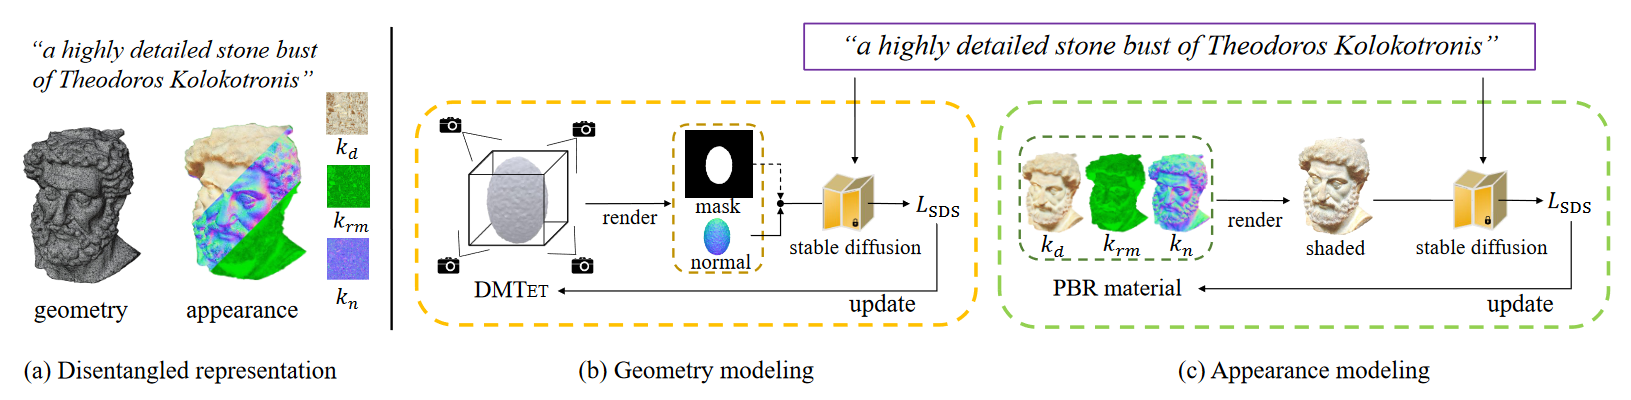
\includegraphics[width=1\columnwidth]{figures/Fantasia3D.png}
      \caption{Summatized functionality of Fantasia3D}\label{fig:figureFantasia3D}
\end{figure}